\chapter{Gestion du projet et choix méthodologique}

\section{Démarches envisagées et démarche retenue}

La conduite d'un projet informatique de l'envergure d'un progiciel de gestion intégré (\emph{ERP}) scolaire multi-établissements impose de choisir une démarche méthodologique garantissant à la fois la conformité fonctionnelle, la rigueur architecturale et la sécurité des données sensibles (notes, paiements, identités).

Deux démarches traditionnelles ont été initialement étudiées :
\begin{enumerate}
    \item \textbf{Le modèle en cascade (cycle en V)} : adapté aux cahiers des charges figés, il offre une traçabilité documentaire forte mais pèche par sa rigidité, retardant excessivement la détection des écarts d'intégration entre le serveur Spring Boot et l'interface React.
    \item \textbf{Les méthodes agiles (Scrum / Kanban)} : axées sur l'itération rapide et les retours utilisateurs fréquents, elles facilitent l'adaptation continue mais risquent, sans outillage de gouvernance strict, de laisser dériver la dette technique ou d'éroder l'étanchéité multi-écoles sous la pression des délais.
\end{enumerate}

Face à ces limites et à la complexité d'un système à acteurs multiples, nous avons retenu une démarche innovante : \textbf{l'Ingénierie Logicielle Agentique Supervisée} (\emph{Supervised Agentic Coding}), combinant un découpage itératif par fonctionnalités et une équipe d'agents d'intelligence artificielle spécialisés encadrés par un superviseur automatisé et un arbitrage humain systématique (\emph{Human-in-the-Loop}). Dans cette approche, aucune ligne de code ni aucun schéma d'API n'est intégré sans franchir des portes de validation formelles (\emph{Quality Gates}).

\section{Mode de gestion et méthode de collecte}

Il convient de distinguer rigoureusement la gouvernance du projet technique de la méthode de collecte et d'analyse des besoins du terrain :
\begin{itemize}
    \item \textbf{Mode de gestion du projet} : le pilotage s'appuie sur une hiérarchie de responsabilités outillée par script (\texttt{orchestrator.sh}). Chaque agent IA se voit assigner une fiche de poste stricte définissant ses livrables autorisés, ses règles bloquantes et ses interdictions formelles. Les échanges entre profils s'effectuent via un bus de communication asynchrone (\texttt{agent\_messages.md}).
    \item \textbf{Méthode de collecte et d'analyse} : l'analyse des besoins s'est fondée sur l'étude des processus administratifs et pédagogiques des établissements sénégalais et ouest-africains (gestion des semestres, coefficients, filières, relevés de notes avec mentions, paiements des droits d'inscription et contrôle des accès par vigile). Les exigences recueillies ont été formalisées sous forme de \emph{User Stories} (\texttt{US-xx}) et de règles métier (\texttt{BR-xx}) consignées dans \nolinkurl{docs/requirements.md}.
\end{itemize}

\section{Rôles, tâches et planification}

\subsection{Répartition des responsabilités et matrice RACI}

Le projet associe des acteurs humains et des profils d'agents spécialisés :
\begin{itemize}
    \item \textbf{Tech Lead humain (Auteur/Étudiant)} : seul décideur, il valide les spécifications, tranche les arbitrages d'architecture, examine les rapports de revue de code et autorise les fusions de branches (\emph{merges}) dans le dépôt principal.
    \item \textbf{Agent 00 — Kasongo (Superviseur)} : contrôle la conformité des livraisons, vérifie le périmètre des fichiers modifiés et émet les visas d'étape (\texttt{audit/kasongo\_report.py}).
    \item \textbf{Agent 01 — Product Analyst} : spécifie les règles métier et les critères d'acceptation Gherkin.
    \item \textbf{Agent 02 — Software Architect} : conçoit l'architecture hexagonale et maintient le contrat unique d'API (\nolinkurl{docs/api-contract.md}).
    \item \textbf{Agent 03 — Backend Developer} : implémente la couche domaine, les adaptateurs JPA et la sécurité Spring Security.
    \item \textbf{Agent 04 — Frontend Developer} : construit l'interface React, les formulaires Zod/React Hook Form et les requêtes TanStack Query.
    \item \textbf{Agent 05 — QA Engineer} : élabore et exécute les suites de tests d'intégration et les scénarios de bout en bout.
    \item \textbf{Agent 06 — Code Reviewer} : réalise l'audit statique, traque les données fictives et vérifie la conformité contractuelle.
    \item \textbf{Agent 07 — DevSecOps Engineer} : audite les dépendances, le cloisonnement Docker et les politiques de sécurité OWASP.
    \item \textbf{Agents 08 à 11} : assurent respectivement la modélisation économique, la rédaction technique, la gestion des releases et la modélisation UML/C4.
\end{itemize}

La figure~\ref{fig:schema-agents} illustre la topologie de collaboration et de supervision stricte reliant les agents, le bus asynchrone et l'arbitrage souverain du Tech Lead.

\begin{figure}[htbp]
  \centering
  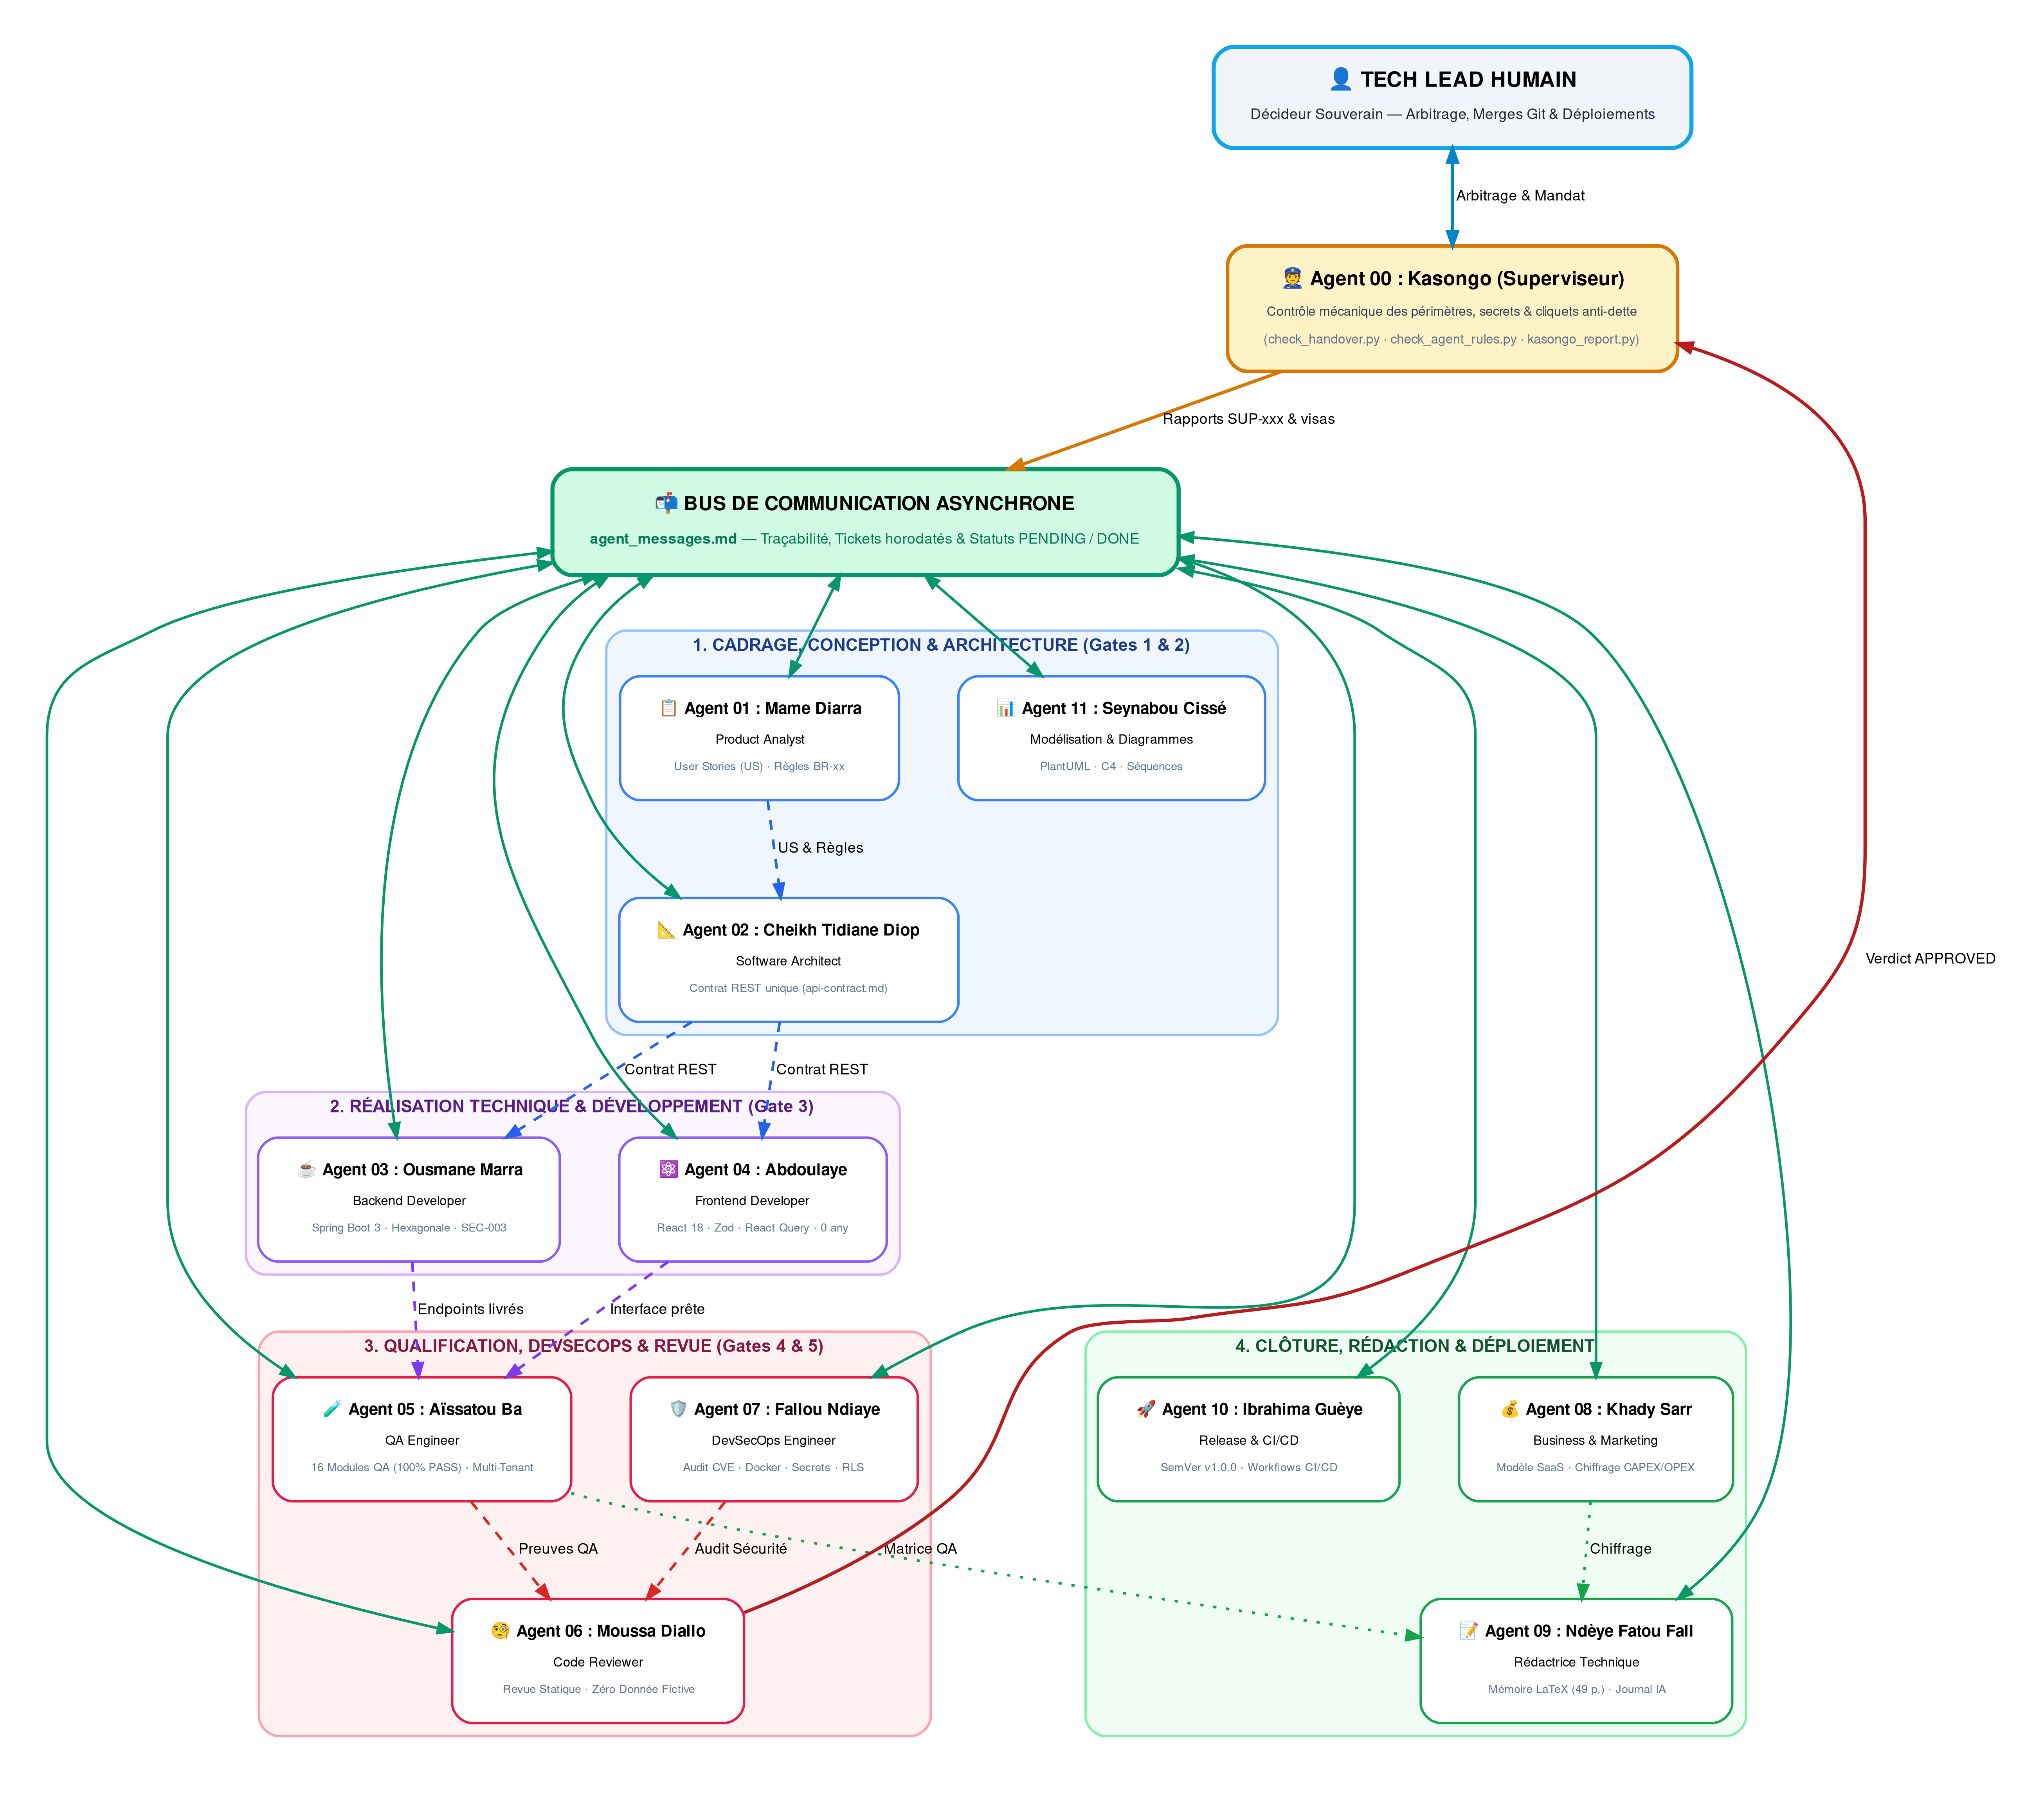
\includegraphics[width=0.98\textwidth]{images/schema-agents.png}
  \caption{Topologie d'interaction et de gouvernance du pipeline multi-agents supervisé}
  \label{fig:schema-agents}
\end{figure}

Le guide exhaustif de portabilité et de réutilisation de ce framework pour d'autres projets logiciels est documenté dans \nolinkurl{docs/guides/framework_agentic_coding.md}.

\subsection{Planification : prévisionnelle vs réalisée}

Le projet a été structuré en cinq jalons clés (\emph{Gates}) :
\begin{table}[h]
\centering
\small
\begin{tabular}{lp{6cm}ll}
\toprule
\textbf{Jalon} & \textbf{Objectif \& Livrable} & \textbf{Statut} & \textbf{Date effective} \\
\midrule
Gate 1 & Cadrage, User Stories \& Règles Métier & Validé & 2026-11-06 \\
Gate 2 & Contrat d'API unique \& Architecture hexagonale & Validé & 2026-11-07 \\
Gate 3 & Réalisation Backend, Frontend \& Isolation multi-tenant & Validé & 2026-11-08 \\
Gate 4 & Qualification QA intégrale (16 modules verts, 100\,\%) & Validé & 2026-11-09 \\
Gate 5 & Revue de code, audit DevSecOps \& Approbation Tech Lead & Validé & 2026-11-09 \\
Post-Gate & Dette frontend (Zod, React Query, suppression \texttt{any}) & Validé & 2026-11-10 \\
\bottomrule
\end{tabular}
\caption{Tableau comparatif des jalons prévus et validés}
\label{tab:jalons-projet}
\end{table}

\section{Outils de suivi et gestion des versions}

La traçabilité absolue des artefacts a reposé sur l'écosystème suivant :
\begin{itemize}
    \item \textbf{Gestion des versions avec Git} : utilisation de branches thématiques (\texttt{feat/*}, \texttt{fix/*}), sous-modules autonomes pour le backend et le frontend, et messages de commit normés selon la convention \emph{Conventional Commits}.
    \item \textbf{Bus d'échange asynchrone (\texttt{agent\_messages.md})} : journal horodaté où chaque agent annonce la publication d'un composant (\texttt{status: PENDING}), les adaptations requises et leur confirmation de réception (\texttt{status: DONE}).
    \item \textbf{Garde-fous automatisés (\texttt{check\_handover.py} \& \texttt{check\_agent\_rules.py})} : scripts d'audit exécutés avant chaque validation pour vérifier le non-dépassement de périmètre, l'absence de fuite de secrets, le respect des cliquets anti-régression (diminution continue des types \texttt{any}) et l'absence totale de l'en-tête interdit \texttt{X-Tenant-Id} côté client.
\end{itemize}

\section{Risques, jalons et gestion des écarts}

Le tableau~\ref{tab:risques-projet} récapitule les risques majeurs identifiés au lancement du projet et les contre-mesures effectives mises en place.

\begin{table}[h]
\centering
\small
\begin{tabular}{lp{4.5cm}p{5.5cm}}
\toprule
\textbf{Risque identifié} & \textbf{Impact potentiel} & \textbf{Mesure préventive appliquée} \\
\midrule
Fuite multi-écoles & Violation de confidentialité critique entre écoles & Intercepteur Spring \texttt{TenantMembershipInterceptor} (SEC-003) + tests d'étanchéité automatisés. \\
Dérive de contrat API & Incompatibilité payload Frontend / Backend & Contrat unique \nolinkurl{docs/api-contract.md} vérifié par \nolinkurl{audit/check_contract_match.py}. \\
Données fictives & Interface présentant de fausses notes ou faux reçus & Remplacement systématique des mocks en dur par des états vides honnêtes et des appels réels. \\
Dette de typage & Instabilité de compilation et plantages à l'exécution & Règle à cliquet R6 réduisant le nombre de \texttt{any} et validation \texttt{tsc -b} avec 0 erreur. \\
\bottomrule
\end{tabular}
\caption{Matrice des risques et contre-mesures associées}
\label{tab:risques-projet}
\end{table}

Chaque écart constaté lors des phases de tests a fait l'objet d'un ticket formel consigné dans le bus, résolu dans le code puis attesté par un fichier de preuve machine (\nolinkurl{docs/evidence/evidence-*.md}).
